% !TeX encoding = UTF-8
\section{Methods}


\subsection{Language Models}
Language Models are computational systems that assign a probability to a word $w_t$ given a sequence of preceding words $w_1, w_2, \dots, w_{t-1}$:
\begin{equation}\label{eq:lm}
    \text{Language Model} = P( w_n | w_1, w_2, \dots, w_{t-1})
\end{equation}
Strictly, LMs operate on tokens and not words. A token is the fundamental unit of text, which can be thought of as word, single character or subword similar to syllables \parencite{sennrich_neural_2016}.
To maintain readability we will use ``word'' instead of ``token''.
All unique words a model can handle are defined as its vocabulary $V$.

A Language Model can also be thought of a system that assigns a probability to a sequence of words $w_1, w_2, \dots, w_t$.
This probability can be factorized into the conditional probability of each word using eq. \ref{eq:lm} and the chain rule:
\begin{equation}
    P(w_1, w_2, \dots, w_t) = \Pi_{i=1}^{t} P( w_i | w_1, w_2, \dots, w_{i-1})
\end{equation}


\subsection{Transformers}
The canonical transformer architecture is characterized by multiple stacks of transformer-blocks, each consisting of a multi-head self-attention layer, feedforward layer, layer normalization and residual connections.
The original transformer introduced in \cite{vaswani_attention_2017} organizes two stacks of transformer-blocks into an encoder and a decoder stack
\footnote{An excellent introduction to transformers can be found in \url{https://nlp.seas.harvard.edu/2018/04/03/attention.html}.}.
Since then, numerous different modifications have been suggested \parencite{tay_efficient_2022}. For instance, \cite{devlin_bert_2019} only use the encoder stack and train their transformer on an adapted version of language modeling. % language modeling is not introduced yet.

The transformers investigated in this thesis use the decoder stack, modeling the conditional distribution of words (eq. \ref{eq:lm}) through successive application of the transformer block to the entire input sequence in parallel  \parencite{radford_improving_2018}:

\begin{equation}\label{eq:transformer}
    \begin{split}
        h_0 &= UW_e + W_p \\
        h_l &= \text{\texttt{transformer\_block}}(h_{l - 1})\quad\forall\; l \in [1,L]\\
        P(w_n | w_1 , \dots , w_{n-1}) &= \texttt{softmax}(h_LW_e^T)
    \end{split}
\end{equation}

where $U = (w_1 , \dots , w_{n-1} )$ is the context vector of words, $L$ is the number of layers, $W_e$ is the word embedding matrix, and $W_p$ is the position embedding matrix.
The transformer block is illustrated in fig \ref{fig:transformer_block}.


\subsection{Language Modeling}
Language modeling (also: causal language modeling) refers to the task of predicting word $w_n$ in context of a preceding sequence of words $w_1, w_2, \dots, w_{n-1}$.
This prediction happens in the form of estimating a probability distribution over $V$.
\begin{equation}
    \text{Probability for $w$ at position $n$ given $w_1, w_2, \dots, w_{n-1}$} = P(w_n | w_1, w_2, \dots, w_{n-1})
\end{equation}
The language model is trained by minimizing the negative log likelihood (NLL)\footnote{Working with the negative log likelihood instead of probabilities has the benefit of numerical stability, as probability values are abysmally small due to large vocabularies in the size of ten-thousands. It is also mathematically valid, because the negative log operation results in a monotonic result that is bigger than 0.} over each word in all sequences $seq$ within the training set $T$:
\begin{equation}
    \text{NLL}(T) = - \frac{1}{|T|} \sum_{\text{seq} \in T} \sum_{w_i \in \text{seq}} \log\left(P(w_i | w_1, w_2, \dots, w_{i-1})\right)
\end{equation}


\subsection{Surprisal}
Formally, the surprisal of a word $w_n$ is defined as the negative log likelihood of the probability that the LM assigns the word $w_n$ at position $n$ given its preceding context $w_1, \dots, w_{n-1}$. It is measured in \textit{bits}:
\begin{equation}
    s(w_n) = - \log_2{P(w_n | w_1, \dots, w_{n-1})}
\end{equation}
In other words, surprisal is used to measure the degree to which a LM ``expected'' the word $w_n$ to occur at position $n$. The higher the surprisal, the less the model has expected to see the word and vice-versa.
In cases when a word is split into multiple sub-words by the byte-pair encoding tokenizer, the surprisal values of the sub-words are summed\footnote{This is valid because the underlying probabilities are not changed: $\log{xy} = \log{x} + \log{y}$}.


\subsection{Paradigm} \label{methods:paradigm}

To test the fWM of a transformer, we present it with a Test-sequence $\text{seq}_T$ and multiple Control-sequences $\text{seq}_{\text{C}} = \left\{ \text{seq}_{\text{C}}^1, \dots, \text{seq}_{\text{C}}^{n_{\text{c}}} \right\}$.
Each Test-sequence is paired with $n_C = 10$ Control-sequences\footnote{We chose $n_C = 10$ because our final measurement stabilizes very quickly, see appendix \ref{app:rs_10_controls}.}, whereby the Test-sequence represents the "Test" and the Control-sequences the "Controls".
Both are jointly constructed.
After construction, we measure the surprisal for each word in the Test-sequence and all Control-sequences:
For every word in a sequence we give all its preceding words as inputs to the transformer and record the surprisal of that word in the output distribution of the transformer.
The surprisal values of Test-sequences are averaged to provide a baseline for the surprisal values in the Test-sequence.
The average from the Test-sequences and the value from the Control-sequence are then finally combined, to obtain a \textit{measure} of repeat surprisal (see \ref{ch:rs}).

\begin{wrapfigure}{L}[0pt]{0pt}
    \centering
    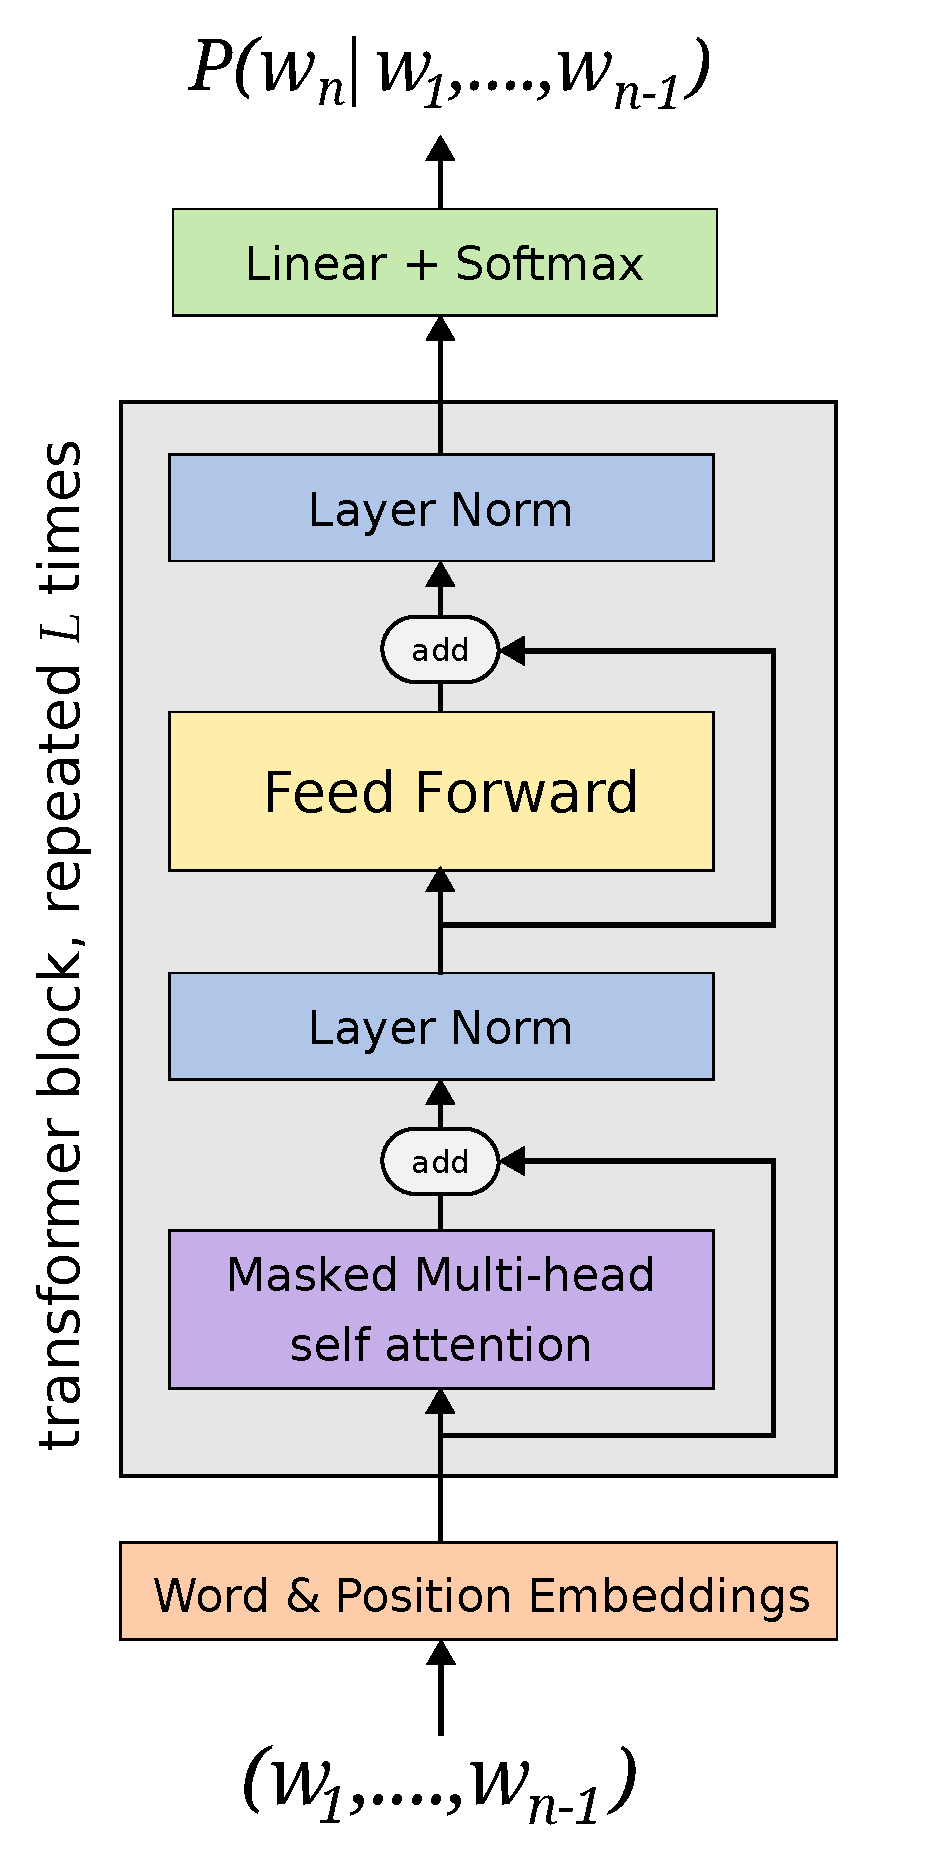
\includegraphics[width=0.4\textwidth]{methods/transformer_block.pdf}
    \caption{Transformer architecture. Input words are embedded and augmented with positional embeddings (orange). The outputs of the embedding layer are fed into the transformer block (grey), which is repeated $L$ times. The last transformer block feeds the outputs into a linear+softmax layer to compute the probability distribution for the next word.}
    \label{fig:transformer_block}
\end{wrapfigure}

The Test-sequence $\text{seq}_T$ and Control-sequences $\text{seq}_{\text{C}}^x$ are constructed from multiple sections:
\begin{center}
    $\text{seq}_{\text{T}}$: \textit{preface}, \textit{encoding-sentence}, \textit{intervention}, \textit{test-sentence}.\\
    $\text{seq}_{\text{C}}^x$: \textit{preface}, \textit{control-sentence}, \textit{intervention}, \textit{test-sentence}.\\
\end{center}
The \textit{preface} is a fixed string that introduces the encoding-sentence (e.g. ``Before the meeting, Mary wrote down the following sentence:'') and is shared by the Test-sequence and the Control-sequence.
In the Test-sequence, the preface is followed by the \textit{encoding-sentence} (e.g. ``the section on current routes adds nothing to the info.'').
The encoding-sentence has a certain relationship with the test-sentence at a later position in the sequence.
In contrast, the \textit{control-sentence} in the Control-sequence is a random sentence that does not have this relationship with the test-sentence (e.g. ``the investigation of chaperones has a long history.'').
At third position follows the \textit{intervention}, a fixed string shared by the Control-sequence and Test-sequence continuing the narrative of the preface and introducing the following section with a short prompt (“After the meeting, Mary took a break. After she got back, she read the sentence again:”).
Finally, the intervention is followed by the \textit{test-sentence} (e.g. “the section on current routes adds nothing to the info.“).

Surprisal reduction on the test-sentence in the Test-sequence would imply that the transformer is able to use the previous context within the Test-sequence to predict the presentation of the test-sentence.
Lack of such surprisal reduction on the test-sentence of the Control-sequence conversely would imply that the transformer cannot use the previous context to predict the presentation of the test-sentence.
As the only difference between the Test-sequence and the Control-sequence are the encoding-sentence and control-sentence, we know that their different relationship to the test-sentence is the source of the surprisal reduction.
This rules out other sources of surprisal reduction which are not related to context, for example the unigram frequency of words within the test-sentence.
Given the appropriate identification of difference in the relationship separating encoding-sentence and control-sentence in respect to the test-sentence, we may now say that the transformer maintained and accessed this relationship in its fWM for next-word-prediction.

The identification of relationships which the fWM of a transformer can use, allows us to characterize the transformers fWM in terms of high-level mechanisms which allow for the use of the feature.
For instance, we may find that the transformers surprisal for the test-sentence is very low when the encoding-sentence is the same as the test-sentence, compared to the surprisal of the test-sentence given a random control-sentence. In such a case, we may denote our feature as "verbatim recall" and describe the fWM of the transformer with a plain copy-paste mechanism.


\subsection{Repeat Surprisal}\label{ch:rs}
In order to quantify the extent to which a LM is able to retrieve specific features from the encoding-sentence (e.g. sentence semantics), we use the notion of \textbf{repeat surprisal}.

We start by taking the surprisal values $\hat{s}$ of the \textit{test-sentence} in the Test-sequence and Control-sequence.
\begin{align}
    \hat{s}\left(\text{seq}_T\right) &:= \left\{\left(w_i, s(w_i)\right) | w_i \in \textit{test-sentence}\;\text{of seq}_T\right\}\\
    \hat{s}\left(\text{seq}_C^x\right) &:= \left\{\left(w_i, s(w_i)\right) | w_i \in \textit{test-sentence}\;\text{of seq}_C^x\right\}
\end{align}
Next, we apply a function $f$ on $\hat{s}$ which yields a scalar.
For instance, $f$ can be the mean, an indexing function returning a specific word or the median:
\begin{equation}\label{eq:f_median}
    f_{\text{median}}\left(\left\{\left(w_1, s(w_1)\right), \dots \right\}\right) := \text{median}\left\{s(w_1), s(w_2), \dots \right\}
\end{equation}
Then, the computed value for a Test-sequence $f\left(\hat{s}\left(\text{seq}_T\right)\right)$ is normalized by the average of the computed values across all the corresponding Control-sequences $f\left(\hat{s}\left(\text{seq}_C^i\right)\right)$.
To yield a percentage, the result is multiplied with 100.
\begin{equation}\label{eq:repeat_surprisal}
    \texttt{repeats surprisal}_f\left(\text{seq}_T, \text{seq}_C\right) := \frac{f\left(\hat{s}\left(\text{seq}_T\right)\right)}{\underset{x}{\text{avg}}\left(f\left(\hat{s}\left(\text{seq}_C^x\right)\right)\right)}\:100
\end{equation}

Here, $f\left(\hat{s}\left(\text{seq}_T\right)\right)$ measures the effect that the encoding-sentence has on the test-sentence.
To make the value interpretable, we divide it by $\underset{i}{\text{avg}}\left(f\left(\hat{s}\left(\text{seq}_C^i\right)\right)\right)$, which measures the average effect any other context (control-sentence) has on the test-sentence.
In other words, $\underset{x}{\text{avg}}\left(f\left(\hat{s}\left(\text{seq}_C^x\right)\right)\right)$ acts as a normalizer for $f\left(\hat{s}\left(\text{seq}_T\right)\right)$.

This method of quantification allows to inspect, in a model agnostic manner, how features of the past context affect the behavior of transformers: by comparing how test-sentence surprisal changes as a function of specific encoding-sentence features, expressed relative to baseline surprisal in control-sentences, we can test what contextual features shape LM's "expectations".
That is, by carefully isolating the target features of the encoding-sentence (e.g. verbatim repetition/identity, semantics, syntax), we can indirectly draw careful conclusions about the transformers fWM capabilities.

The repeat surprisal has the useful quality that it ensures it is in fact a specific feature of the encoding-sentence in respect to the test-sentence which drives the effect on repeat surprisal instead of properties of the vignette (preface, intervention) or test-sentence itself.
For example, if a feature of the vignette (e.g. the intervention's length) or a feature of the test-sentence (e.g. it contains highly probable words) have an impact on surprisal values (and they certainly do), these features will affect \textbf{both} the Test-sequence and the Control-sequences similarly, cancelling out in the division in eq. \ref{eq:repeat_surprisal}.
For this reason, only the \textbf{difference in features} between encoding-sentence and control-sentences in respect to test-sentence is driving the effect.

\begin{figure}
    \centering
    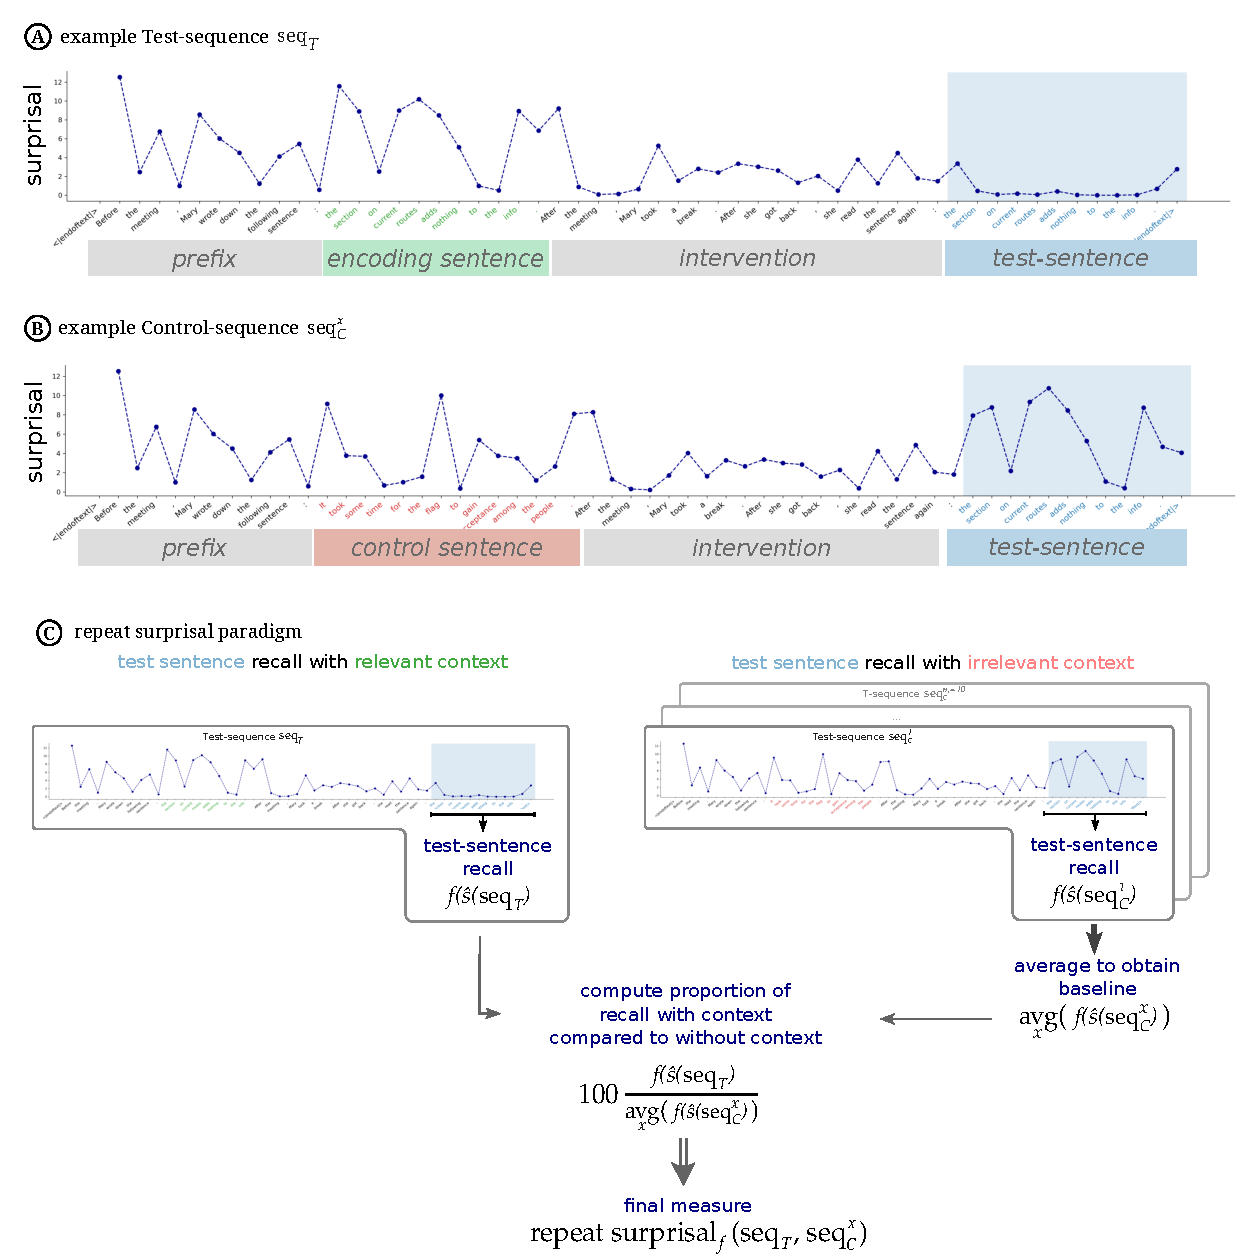
\includegraphics[width=\textwidth]{methods/paradigm.pdf}
    \caption{The paradigm and example surprisal plots. \textbf{A}: Example Test-sequence $\text{seq}_T$: \textit{preface} (grey), \textit{encoding-sentence} (green), \textit{intervention} (grey), \textit{test-sentence} (blue). \textbf{B}: Example Control-sequence $\text{seq}_C^x$ : \textit{preface}, \textit{control-sentence} (red), \textit{intervention}, \textit{test-sentence}. \textbf{C}: Repeat surprisal computation with Test-sequence $\text{seq}_T$ and Control-sequence $\text{seq}_C^x$. From the surprisal values of the test-sentence a single value is computed with $f$. For the Control-sequences these are averaged. The result from the Test-sequence is divided by the averaged result of the Control-sequences and multiplied by 100 to obtain one \textit{measure} of repeat surprisal.}
\end{figure}


\subsection{Repeat Surprisal interpretation}
Given the Test-sequence and Control-sequence, the repeat surprisal has some general implications:

\paragraph{A repeat surprisal percentage close to 0}
indicates that the encoding-sentence provides the LM's WM with context which leads the model to strongly "expect" the test-sentence, whilst the control-sentence does not provide such context.
The encoding-sentence contains some relevant feature to predict the test-sentence, and - importantly - the LM is able to extract and use that feature in its WM.
It is not necessary that the feature aligns with the intuition of a human observer.

\paragraph{A repeat surprisal percentage below 100, but not close to 0}
indicates that the LM is able to extract the relevant information from the encoding-sentence to be less surprised at presentation of the test-sentence, but this information is not definitive enough to make the model strongly expect the test-sentence. This is not necessarily a sign that the model is failing to extract some feature, but instead indicates that the model distributes its expectation over multiple possible test-sentences. Again, the feature the model extracts does not have to align with human intuition.
\paragraph{A repeat surprisal percentage at/around 100}
indicates the LM is not able to extract any relevant information from the given encoding-sentence to predict the test-sentence. In other words, to the LM the encoding-sentence provides as little information as the control sentences. In the case in which a human observer can use some feature from the encoding-sentence in order to be less surprised at presentation of the test-sentence, we can deduce that the model is unable to extract such a feature in at least some cases. The more data points of such nature we collect, the more we can conclude the LM's WM is not capable of operating with such a feature in the encoding-sentence. % a bit more careful here probably. Maybe add "for certain situations"
\paragraph{A repeat surprisal percentage over 100}
indicates the LM is able to extract relevant information from the encoding sentence to \textit{not} expect the test-sentence. In other words, the feature used by the LM's WM encodes something significantly different from what is given in the test-sentence. Again, such an observation may or may not align with human intuition.


\subsection{Sentences used}\label{met:sentences_used}

\paragraph{nonce-sentences}
The first source for the used sentences is the nonce stimulus dataset \cite{wei_frequency_2021} - a dataset containing 300 nouns, 200 verbs and 57 sentence templates.
Each template has one correct noun and verb pair associated with it.
The sentences were revised and filtered, such that in the end we are left with 35 syntactically correct and semantically plausible sentences.
Each sentence has a marked verb and noun. For examples, see \ref{ap:nonce_sentences}.

\paragraph{wikitext sentences}
To introduce a more diverse set of sentences, we used a second set of sentences.
These sentences are sampled from Wikitext103 \parencite{merity_pointer_2016}.
Verbs and nouns were pre-marked with \parencite{van_nguyen_trankit_2021} and then revised and filtered, such that we supplement our pool of sentences by another 25 sentences.

\subsection{Transformers used}

The models are chosen to include varying model sizes and cover different levels of performance.
An overview is provided in table \ref{Tab:models_used}. We used the Hugging Face library \parencite{wolf_transformers_2020}\footnote{\url{https://huggingface.co/}} to access the transformers.\\
\\
\textbf{distilGPT2} is a small version of the same architecture as GPT2. It was trained with GPT2 as supervisor on 38GB of the OpenWebTextCorpus \parencite{gokaslan_openwebtext_2019}. \\
\textbf{GPT2} is a model published by OpenAI mainly based on GPT \parencite{radford_language_2019}.
It uses only the decoder part of the original Transformer.
GPT2 is trained with a LM objective on 40GB of data mined from the internet.
In addition to its base version we used \textbf{GPT2-medium} and \textbf{GPT2-large} as well.
Both differ in their parameter size and amount of transformer block layers to GPT2.\\
\textbf{GPT-neo} is the open source implementation of GPT3.
It is similar in architecture to GPT2, but vastly bigger in size.
GPT-neo is trained on ``The Pile'' \parencite{gao_pile_2020}, a massive dataset of 800GB extracted from the internet with an emphasis on bias and fairness.\\

\begin{table} \centering
    \begin{threeparttable}
        \begin{tabular}{l c c c c }
            \hline
            \thead{Transformer} & \thead{Training\\corpus size}&\thead{Parameters \\ \#} & \thead{WikiText103 \\ (PPL)} \\
            \hline\hline
             distilGPT2     & 38GB & 82M & -\tnote{++}\\
             GPT2-base     & 40GB & 117M & 37.50\tnote{+}\\
             GPT2-medium   & 40GB & 345M & 26.37\tnote{+}\\
             GPT2-large    & 40GB & 762M & 22.05\tnote{+}\\
             GPT-neo & 800GB & 1.3B & 13.10\tnote{*}\\
             \hline
        \end{tabular}
        \begin{tablenotes}\footnotesize
            \item[+] from \textcite{radford_language_2019}
            \item[*] from \url{https://github.com/EleutherAI/gpt-neo/}
            \item[++] ppl without fine-tuning not reported by model creators
        \end{tablenotes}
        \caption{The different pretrained transformers tested in our experiments. They mainly differ in their number of parameters and training corpus size. All transformers are based on the decoder-only architecture \parencite{radford_improving_2018}.} \label{Tab:models_used}
    \end{threeparttable}
\end{table}\textbf{}

\subsection{Implementation}

The entire code to replicate the results and the raw data for each experiment are available at the following github repository: \url{https://github.com/GabrielKP/transformer_wm}.

The implementation is based on an ongoing private codebase from Kristijan Armeni. We realized the project in python, using pytorch \parencite{paszke_pytorch_2019_correct} as neural network framework and the huggingface library \parencite{wolf_transformers_2020} to access transformers. We use numpy \parencite{harris_array_2020_correct} for vectorized operations and pandas \parencite{reback_the_2020_correct} for data management. Plots are created with seaborn \parencite{waskom_seaborn_2021_correct} and matplotlib \parencite{hunter_matplotlib_2007_correct}.

\newpage
